% Options for packages loaded elsewhere
\PassOptionsToPackage{unicode}{hyperref}
\PassOptionsToPackage{hyphens}{url}
%
\documentclass[
]{article}
\usepackage[margin= 1.5 in]{geometry}
%\usepackage{lastpage}
%\usepackage{fancyhdr}
%\pagestyle{fancy} 
\usepackage{lmodern}
\usepackage{amssymb,amsmath}
\usepackage{ifxetex,ifluatex}
\ifnum 0\ifxetex 1\fi\ifluatex 1\fi=0 % if pdftex
  \usepackage[T1]{fontenc}
  \usepackage[utf8]{inputenc}
  \usepackage{textcomp} % provide euro and other symbols
\else % if luatex or xetex
  \usepackage{unicode-math}
  \defaultfontfeatures{Scale=MatchLowercase}
  \defaultfontfeatures[\rmfamily]{Ligatures=TeX,Scale=1}
\fi
% Use upquote if available, for straight quotes in verbatim environments
\IfFileExists{upquote.sty}{\usepackage{upquote}}{}
\IfFileExists{microtype.sty}{% use microtype if available
  \usepackage[]{microtype}
  \UseMicrotypeSet[protrusion]{basicmath} % disable protrusion for tt fonts
}{}
\makeatletter
\@ifundefined{KOMAClassName}{% if non-KOMA class
  \IfFileExists{parskip.sty}{%
    \usepackage{parskip}
  }{% else
    \setlength{\parindent}{0pt}
    \setlength{\parskip}{6pt plus 2pt minus 1pt}}
}{% if KOMA class
  \KOMAoptions{parskip=half}}
\makeatother
\usepackage{xcolor}
\IfFileExists{xurl.sty}{\usepackage{xurl}}{} % add URL line breaks if available
\IfFileExists{bookmark.sty}{\usepackage{bookmark}}{\usepackage{hyperref}}
\hypersetup{
  hidelinks,
  pdfcreator={LaTeX via pandoc}}
\urlstyle{same} % disable monospaced font for URLs
\usepackage{graphicx,grffile}
\makeatletter
\def\maxwidth{\ifdim\Gin@nat@width>\linewidth\linewidth\else\Gin@nat@width\fi}
\def\maxheight{\ifdim\Gin@nat@height>\textheight\textheight\else\Gin@nat@height\fi}
\makeatother
% Scale images if necessary, so that they will not overflow the page
% margins by default, and it is still possible to overwrite the defaults
% using explicit options in \includegraphics[width, height, ...]{}
\setkeys{Gin}{width=\maxwidth,height=\maxheight,keepaspectratio}
% Set default figure placement to htbp
\makeatletter
\def\fps@figure{htbp}
\makeatother
\setlength{\emergencystretch}{3em} % prevent overfull lines
\providecommand{\tightlist}{%
  \setlength{\itemsep}{0pt}\setlength{\parskip}{0pt}}
\setcounter{secnumdepth}{-\maxdimen} % remove section numbering

\date{}

\begin{document}

\hypertarget{header-n3879}{%
\section{(05) Continuity}\label{header-n3879}}

Wk 4 Material; Topic 3; Due 28 March

\tableofcontents

\newpage
\hypertarget{header-n3882}{%
\subsection{Continuous Functions {[}5.1{]}}\label{header-n3882}}

\hypertarget{header-n3883}{%
\subsubsection{Definition of Continuity}\label{header-n3883}}

Take some function \(f: A \rightarrow B\) where
\(A \subseteq \mathbb{R}\):

\begin{itemize}
\item
  the function \(f\) is said to be continuous at some point \(c\in A\)
  if and only if \(\lim_{x\rightarrow c} = f(c)\)
\end{itemize}

\hypertarget{header-n3888}{%
\paragraph{Rigorous Definition}\label{header-n3888}}

So let's phrase that using the \(\varepsilon\)-\(\delta\) definition of
the limit:

\begin{figure}
\centering
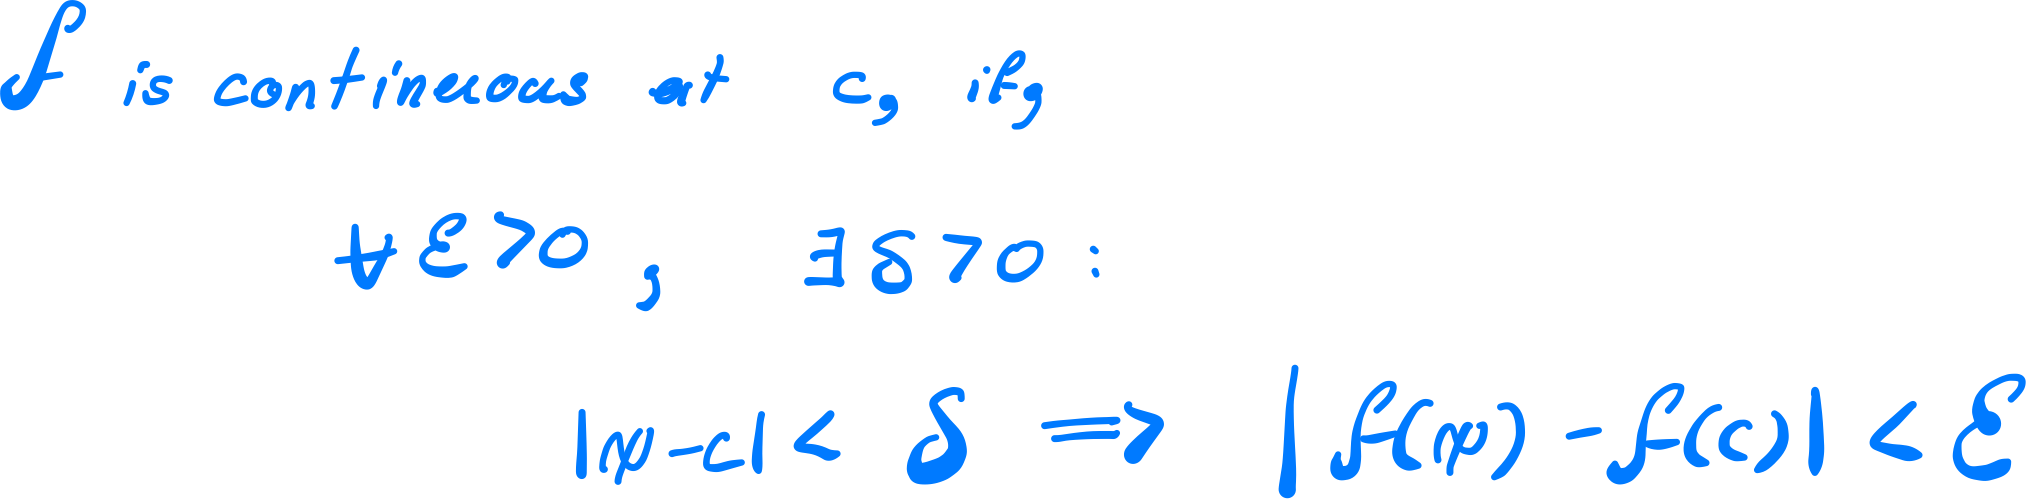
\includegraphics{/home/ryan/Dropbox/Analysis/MD_Working_Directory/05_Continuity/5a4384a9f2a06610556cce9d4252fedc2d5050eb.png}
\caption{}
\end{figure}

\hypertarget{header-n3891}{%
\subparagraph{In Terms of Neighborhoods}\label{header-n3891}}

This can be expressed in terms of neighborhoods:
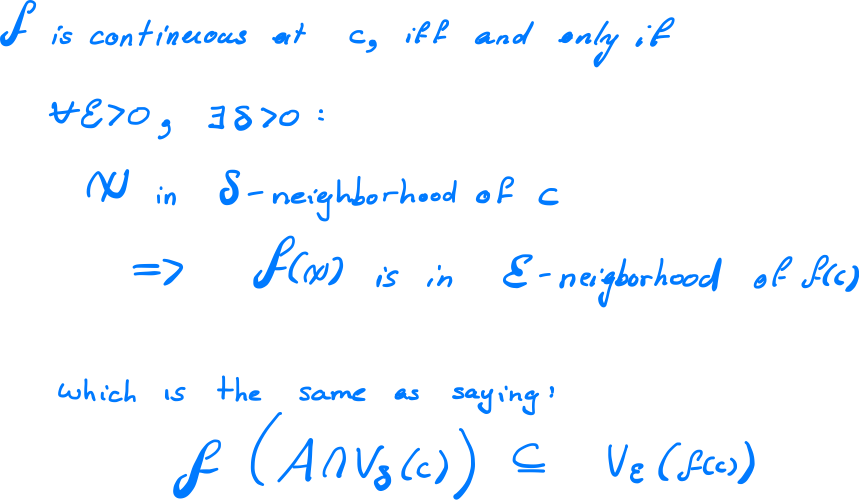
\includegraphics{/home/ryan/Dropbox/Analysis/MD_Working_Directory/05_Continuity/6d89890c4876af9738ff2bd73575f425a45c101a.png}

\newpage
\hypertarget{header-n3893}{%
\paragraph{Conditions for Continuity}\label{header-n3893}}

If \(c\) is a cluster point of \(A\), then trhee conditions must hold
for \(f\) to be continuous at \(c\), that is to say that three
conditions must hold for \(\lim_{x\rightarrow c} = f(c)\):

\begin{enumerate}
\def\labelenumi{\arabic{enumi}.}
\item
  \(f\) must be defined at \(c\)

  \begin{itemize}
  \item
    so that \(f(c)\) actually has meaning
  \end{itemize}
\item
  The limit of \(f\) at \(c\) must exist in \(\mathbb{R}\) so that

  \begin{itemize}
  \item
    \(\lim_{x\rightarrow c}\) actually has a meaning
  \end{itemize}
\item
  These two values are equal

  \begin{itemize}
  \item
    \(\lim_{x\rightarrow c} = f(c)\)
  \end{itemize}
\end{enumerate}

\begin{quote}
\textbf{\emph{Cluster Points}}

A cluster point has infinitely divisible values either side of it, if a
value is not a cluster point it's just an isolated point and it is said
to be continuous at that point, so generally we just assume points are
cluster points because if they're not then they're automatically
continuous and so not very interesting.
\end{quote}

\hypertarget{header-n3914}{%
\subsubsection{Sequential Criterion for Continuity
{[}5.1.3{]}}\label{header-n3914}}

Just like a limits can be defined in terms of sequences (at (4.1.8) of
the TB), continuity can hence be defined in terms of sequences:

A function \(f: A \rightarrow \mathbb{R}\) is continuous at some point
\(c \in A \) if and only if:

\begin{itemize}
\item
  for every sequence \((x_n)\) in \(A\) that converges to \(c\)

  \begin{itemize}
  \item
    \(f\left(\left( x_n \right) \right)\) converges to \(c\) 
  \end{itemize}
\end{itemize}

\hypertarget{header-n3923}{%
\paragraph{Discontinuity Criterion {[}5.1.4{]}}\label{header-n3923}}

Just like limits can have divergence criteria in terms of limits, so can
the continuity definition, this is analogous to the \emph{Limit
Divergence Criteria} at (4.1.9(a) of the TB).

A function \(f: A \rightarrow \mathbb{R}\) is \textbf{discontinuous} at
some point \(c \in A \) if and only if:

\begin{itemize}
\item
  there exists some sequence \((x_n)\) in \(A\) that converges to \(c\):

  \begin{itemize}
  \item
    \(f\left(\left( x_n \right) \right)\) \emph{*does note} converge to
    \(c\) 
  \end{itemize}
\end{itemize}

\hypertarget{header-n3932}{%
\subparagraph{Example}\label{header-n3932}}

\(\lim_{x\rightarrow 0} \sin(\frac{1}{x^2})\) is undefined, so a
sequence that converges to 0 does is such that
\(f\left(\left( x_n \right) \right)\) \emph{*does note} converge to
\(c\) and so by (5.1.4) we can conclude that the function is
discontinuous at 0.

\hypertarget{header-n3934}{%
\subsubsection{Set Continuity}\label{header-n3934}}

if \(B\) is a subset of \(A\) we can say that the function
\(f: A \rightarrow B \) is continuous on \(B\) if it is continuous at
every point on \(B\).

\hypertarget{header-n3936}{%
\subsubsection{Defining a function to overcome
Discontinuity}\label{header-n3936}}

So take a function that is discontinuous, e.g.
\(\enspace f(x) = \frac{x^2-1^2}{(x+1)\cdot (x-1)}\) is discontinuous at
\(x = \pm 1\), to overcome this we can define a anew function \(g(x)\):

\[g(x) = 
  \begin{cases}
    f\left( x \right) , \enspace
   x\neq \pm1\\ 
   1\quad \enspace \enspace  , \enspace   x = \pm 1\\
      \end{cases}\]

This function will be continuous because the 'hole' is more or less
'plugged' by a given value.

\begin{itemize}
\item
  if there is no limit value at the discontinuity, then obviously this
  method won't work because we have no value with which to 'plug' the
  'hole'
\end{itemize}

\hypertarget{header-n3943}{%
\subsection{Combinations of Continuous Functions
{[}5.2{]}}\label{header-n3943}}

\hypertarget{header-n3944}{%
\subsubsection{Absolute Values Preserve Continuity
(5.2.4)}\label{header-n3944}}

Take our function \(f: A \rightarrow B\) and define the absolute
function as :

\begin{itemize}
\item
  \(\text{abs}(f)(x) = \left| f \right|(x) := \left| f(x) \right| \qquad\forall x \in A\)

  \begin{itemize}
  \item
    If \(f\) is continuous at \(c\), then \(\left| f(x) \right|\) is
    continuous at \(c\) 
  \item
    If \(f\) is continuous on \(A\), then \(\left| f(x) \right|\) is
    continuous on \(A\) 
  \end{itemize}
\end{itemize}

\hypertarget{header-n3954}{%
\subsubsection{Square Roots Preserve Continuity}\label{header-n3954}}

Take our function \(f: A \rightarrow B\) and define the square root
function as :

\begin{itemize}
\item
  \(\text{sqrt}(f)(x) = \left(\sqrt{(f)}\right) \left(x\right) := \sqrt{f(x)} \qquad\forall x \in A\)

  \begin{itemize}
  \item
    If \(f\) is continuous at \(c\), then
    \( \left(\sqrt{(f)}\right) \left(x\right)\) is continuous at \(c\) 
  \item
    If \(f\) is continuous on \(A\), then
    \( \left(\sqrt{(f)}\right) \left(x\right)\) is continuous on \(A\) 
  \end{itemize}
\end{itemize}

\hypertarget{header-n3964}{%
\subsubsection{Compositions Preserve Continuity}\label{header-n3964}}

Let:

\begin{itemize}
\item
  \(A, B \subseteq R\)

  \begin{itemize}
  \item
    \(f: A \rightarrow B\) 
  \item
    \(g: B\rightarrow \mathbb{R}\)

    \begin{itemize}
    \item
      \(f(A) \subseteq \mathbb{R}\) 
    \end{itemize}
  \end{itemize}
\end{itemize}

If \(f\) is continuous at \(c\) and \(g\) continuous at \(f(c)\) then
\(g\left( f\left( x\right) \right) = \left(g \circ f \right): A \rightarrow \mathbb{R}\)
is continuous at \(c\)

If \(f\) is continuous on \(A\) and \(g\) continuous on \(B\) then
\(g\left( f\left( x\right) \right) = \left(g \circ f \right): A \rightarrow \mathbb{R}\)
is continuous on \(A\)

\hypertarget{header-n3979}{%
\subsection{Continuous Functions on Intervals
{[}5.3{]}}\label{header-n3979}}

These weren't in the lecture Notes, they're probably not too important.

\hypertarget{header-n3981}{%
\subsection{Uniform continuity {[}5.4{]}}\label{header-n3981}}

These weren't in the lecture Notes, they're probably not too important.

\hypertarget{header-n3984}{%
\subsection{The Mean Value Theorem {[}6.2{]}}\label{header-n3984}}

\hypertarget{header-n3985}{%
\subsubsection{Maximum / Minimum {[}6.2.0{]}}\label{header-n3985}}

Take some function \(f: I \rightarrow \mathbb{R}\)

\begin{itemize}
\item
  \(f\) has a relative \textbf{maximum} if there exists some
  neighbourhood \(V:=V_{\delta}\left( c \right)\) such that::

  \begin{itemize}
  \item
    \(f(x) \geq f(c) \quad \forall x \in \left( V\cap I \right)\)
  \end{itemize}
\item
  \(f\) has a relative \textbf{minimum} if there exists some
  neighbourhood \(V:=V_{\delta}\left( c \right)\) such that:

  \begin{itemize}
  \item
    \(f(x) \leq f(c) \quad \forall x \in \left( V\cap I \right)\)
  \end{itemize}
\end{itemize}

If either of these are satisfied then \(f\) is said to have a
\textbf{relative extrema}

\hypertarget{header-n3999}{%
\subsubsection{Interior Extrema Theorem
{[}6.2.1{]}}\label{header-n3999}}

let \(c\) be a point on some interval \(I\) at which \(f\) has a max/min

\begin{itemize}
\item
  If there is a derivative at \(c\) then it must be 0:

  \begin{itemize}
  \item
    \(c\) is a point of at which \(f\) has a \emph{relative extremum}
    \(\implies\) \(f^{\prime}(c)=0\)
  \end{itemize}
\item
  The derivative at \(c\) must be 0 or must be undefined.

  \begin{itemize}
  \item
    \(f'(c) = 0 \vee f'(c) \in \emptyset\)
  \item
    \(f'(c) = 0 \vee f'(c) \downarrow\)
  \end{itemize}
\end{itemize}

In \emph{Computability: An Introduction to Recursion Theory} 1 the
\(\downarrow\) symbol is said to mean undefined, it's a useful notation
so I've adopted it, \(\in \emptyset\) is potentially another technique
as well.

\newpage
\hypertarget{header-n4017}{%
\subsubsection{Rolle's Theorem {[}6.2.3{]}}\label{header-n4017}}

Suppose that:

\begin{itemize}
\item
  \(f\) is continuous on \(I:= [a,b]\)
\item
  \(f'\) exists at every point of the open interval \((a,b)\)
\item
  \(f(a) = f(b) = 0\)
\end{itemize}

Then there must exist some value \(c\) such that \(f'(c) = 0\)

\begin{itemize}
\item
  This is the same as saying there must be a point of relative extrema
  (by the \emph{Interior Extrema Theorem})
\end{itemize}

\begin{figure}
\centering
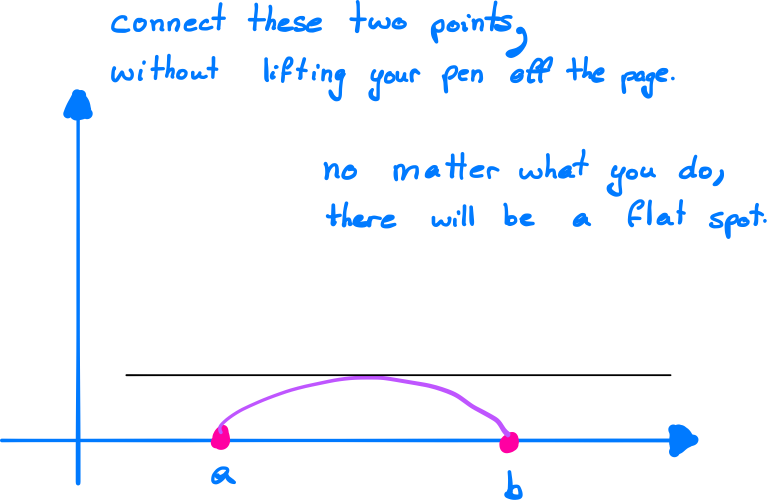
\includegraphics[width=0.7\columnwidth]{/home/ryan/Dropbox/Analysis/MD_Working_Directory/05_Continuity/f90f9756a7cc0b3ce971b414fb96a5f04d7c53dd.png}
\caption{}
\end{figure}

\begin{figure}
\centering
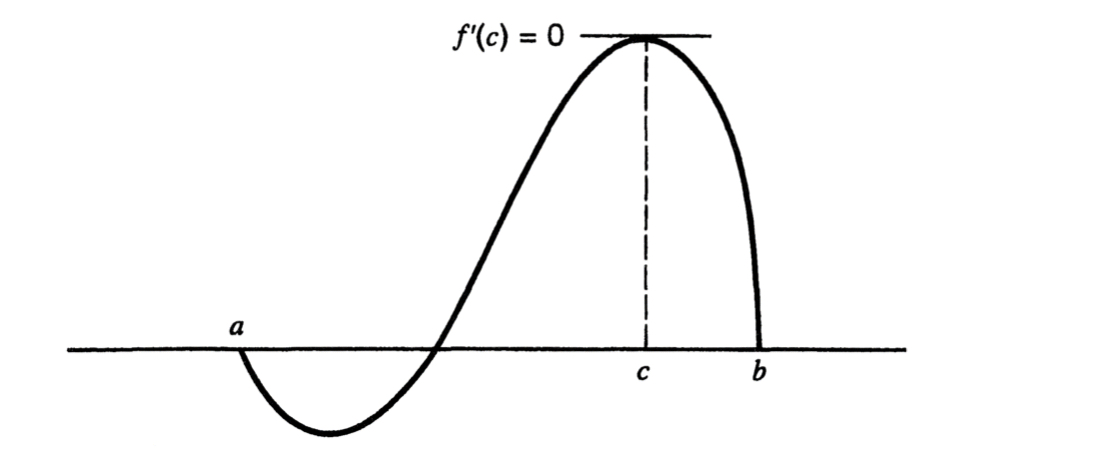
\includegraphics{/home/ryan/Dropbox/Analysis/MD_Working_Directory/05_Continuity/E744A1A9-00E0-4C46-971D-CE0A063D7664.jpeg}
\caption{}
\end{figure}

\hypertarget{header-n4032}{%
\subsubsection{Mean Value Theorem {[}6.2.4{]} }\label{header-n4032}}

This is basically a built up version of Rolle's Theorem,

Suppose that:

\begin{itemize}
\item
  \(f\) is continuous on \(I:= [a,b]\)
\item
  \(f'\) exists at every point of the open interval \((a,b)\)
\end{itemize}

Then, there must exist some \(c\):

\[f'\left( c \right) = \frac{f\left( b \right)-f\left( a \right)}{b-a} \\
\implies  \left( b-a \right) \cdot f\left( c \right) = f\left( b \right) - f\left( a \right)\]

\begin{figure}
\centering
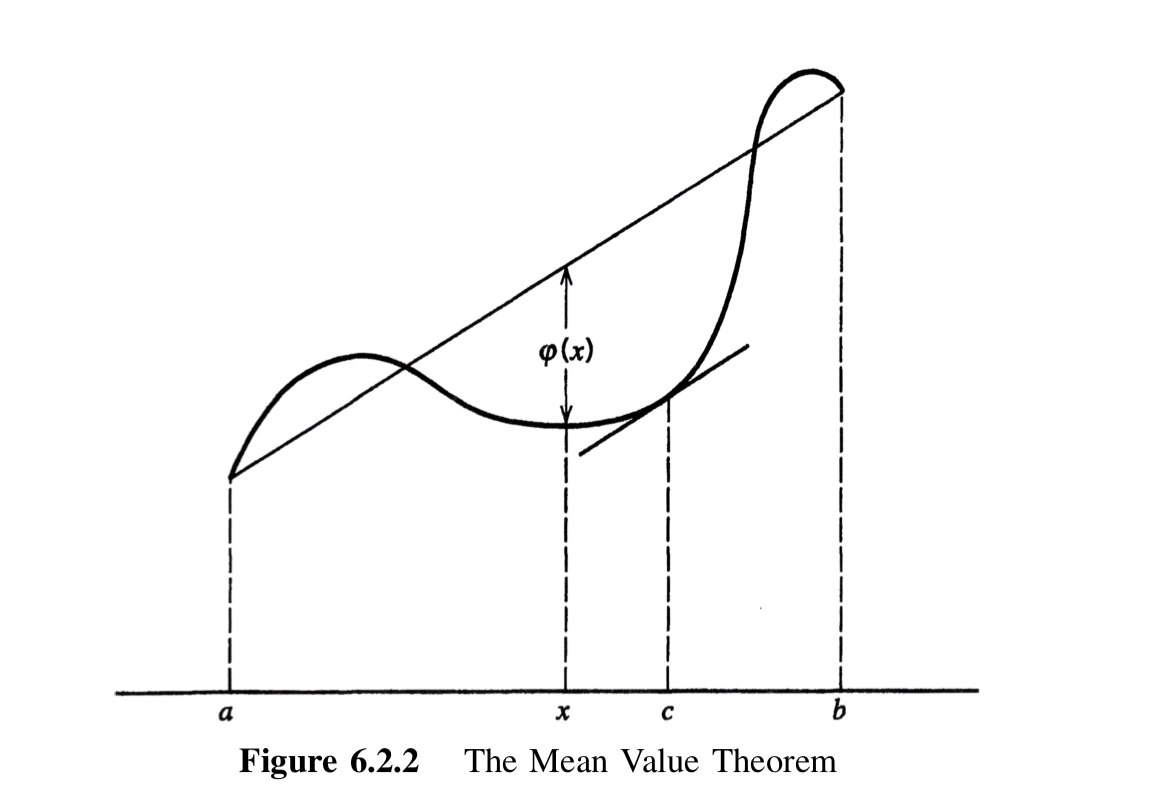
\includegraphics[width=0.7\columnwidth]{/home/ryan/Dropbox/Analysis/MD_Working_Directory/05_Continuity/3256156E-84DC-4942-B3D3-B580180EEE50.jpeg}
\caption{}
\end{figure}

\newpage
\hypertarget{header-n4043}{%
\subsection{L'Hospital's Rules}\label{header-n4043}}

\hypertarget{header-n4044}{%
\subsubsection{Cauchy Mean Value Theorem}\label{header-n4044}}

let \(f\) and \(g\) be:

\begin{itemize}
\item
  Continuous on {[}a,b{]}
\item
  Differentiable on (a,b)
\end{itemize}

if \(g'(x)  \neq 0\) , then \(\exists c \in (a,b)\) :

\[\frac{f\left( b \right)-f\left( a \right)}{g\left( b \right) - g\left( a \right)} = \frac{f'\left( c \right)}{g'\left( c \right)}\]

\hypertarget{header-n4054}{%
\paragraph{Restrictions}\label{header-n4054}}

By \emph{Rolle's Theorem}, if \(g'(x) \neq 0\), then \(g(a) \neq g(b)\).

\hypertarget{header-n4056}{%
\subparagraph{Creating a stricter restriction}\label{header-n4056}}

Let's suppose for some reason you needed to create the restriction:

\begin{itemize}
\item
  \(g'(x) \neq 0\), and
\item
  \(g(a) \neq g(b)\) 
\end{itemize}

An equivalent restriction would be:

\[\left( f'\left( x \right) \right)^{2} + \left( g'\left( x \right) \right)^{2} \neq 0\]


\end{document}
